\documentclass[a4paper,11pt]{article}

\usepackage[margin=2.5cm]{geometry}
\usepackage[utf8]{inputenc}
\usepackage[colorlinks=true,allcolors=blue]{hyperref}
\usepackage{amsmath}
\usepackage{graphicx}
\usepackage{float}
\usepackage{caption}
\usepackage{subcaption}
\usepackage{xcolor}
%\usepackage{listings} %Alternative to minted
\usepackage{listings}

\lstset{
aboveskip=0.5\baselineskip,
belowskip=0.5\baselineskip
}
\definecolor{codegreen}{rgb}{0,0.6,0}
\definecolor{codegray}{rgb}{0.5,0.5,0.5}
\definecolor{codepurple}{rgb}{0.58,0,0.82}
\definecolor{backcolour}{rgb}{0.95,0.95,0.92}
\lstdefinestyle{mystyle}{
backgroundcolor=\color{backcolour},
commentstyle=\color{codegreen},
keywordstyle=\color{magenta},
numberstyle=\tiny\color{codegray},
stringstyle=\color{codepurple},
basicstyle=\footnotesize\ttfamily,
breakatwhitespace=false,
breaklines=true, captionpos=b,
keepspaces=true, numbers=left,
numbersep=5pt, showspaces=false,
showstringspaces=false,
showtabs=false, tabsize=2,
}
\lstset{style=mystyle,
basicstyle=\ttfamily\footnotesize, % Use monospaced font and smaller size
keywordstyle=\color{blue},        % Keywords in blue
stringstyle=\color{red},          % Strings in red
commentstyle=\color{gray},        % Comments in gray
showstringspaces=false,            % Do not show spaces in strings
frame=single,                      % Frame the code block
numbers=left,                      % Line numbers on the left
numberstyle=\tiny\color{gray},   % Line numbers style
breaklines=true,                   % Line breaks for long lines
backgroundcolor=\color{lightgray!20}, % Light gray background
}
\setlength{\parindent}{0em}
\setlength{\parskip}{1em}

\title{\textbf{Hand-in Assignment 1} \\ Analysis of Time Series 1MS014}
\author{Aditya Khadkikar, Aviral Jain}
\date{\today}

\begin{document}
    \maketitle
    \section*{Task 4}
    The number of registered private cars in Sweden for the years 1977 until February 2025, monthly data, is given in the second column of the file carsmon.dat at Studium. 
    
    Find a suitable ARIMA (or SARIMA) model for these data, or a transformation thereof. Analyze the model residuals carefully, in order to make sure that the model provides a good description of the data. It might be a good idea to try transformations, like the logarithm. \\
    
    \hrule

    Below is the time-series data plotted for the dataset of registered private cars from 1977-2025:

    \begin{figure}[H]
        \centering
        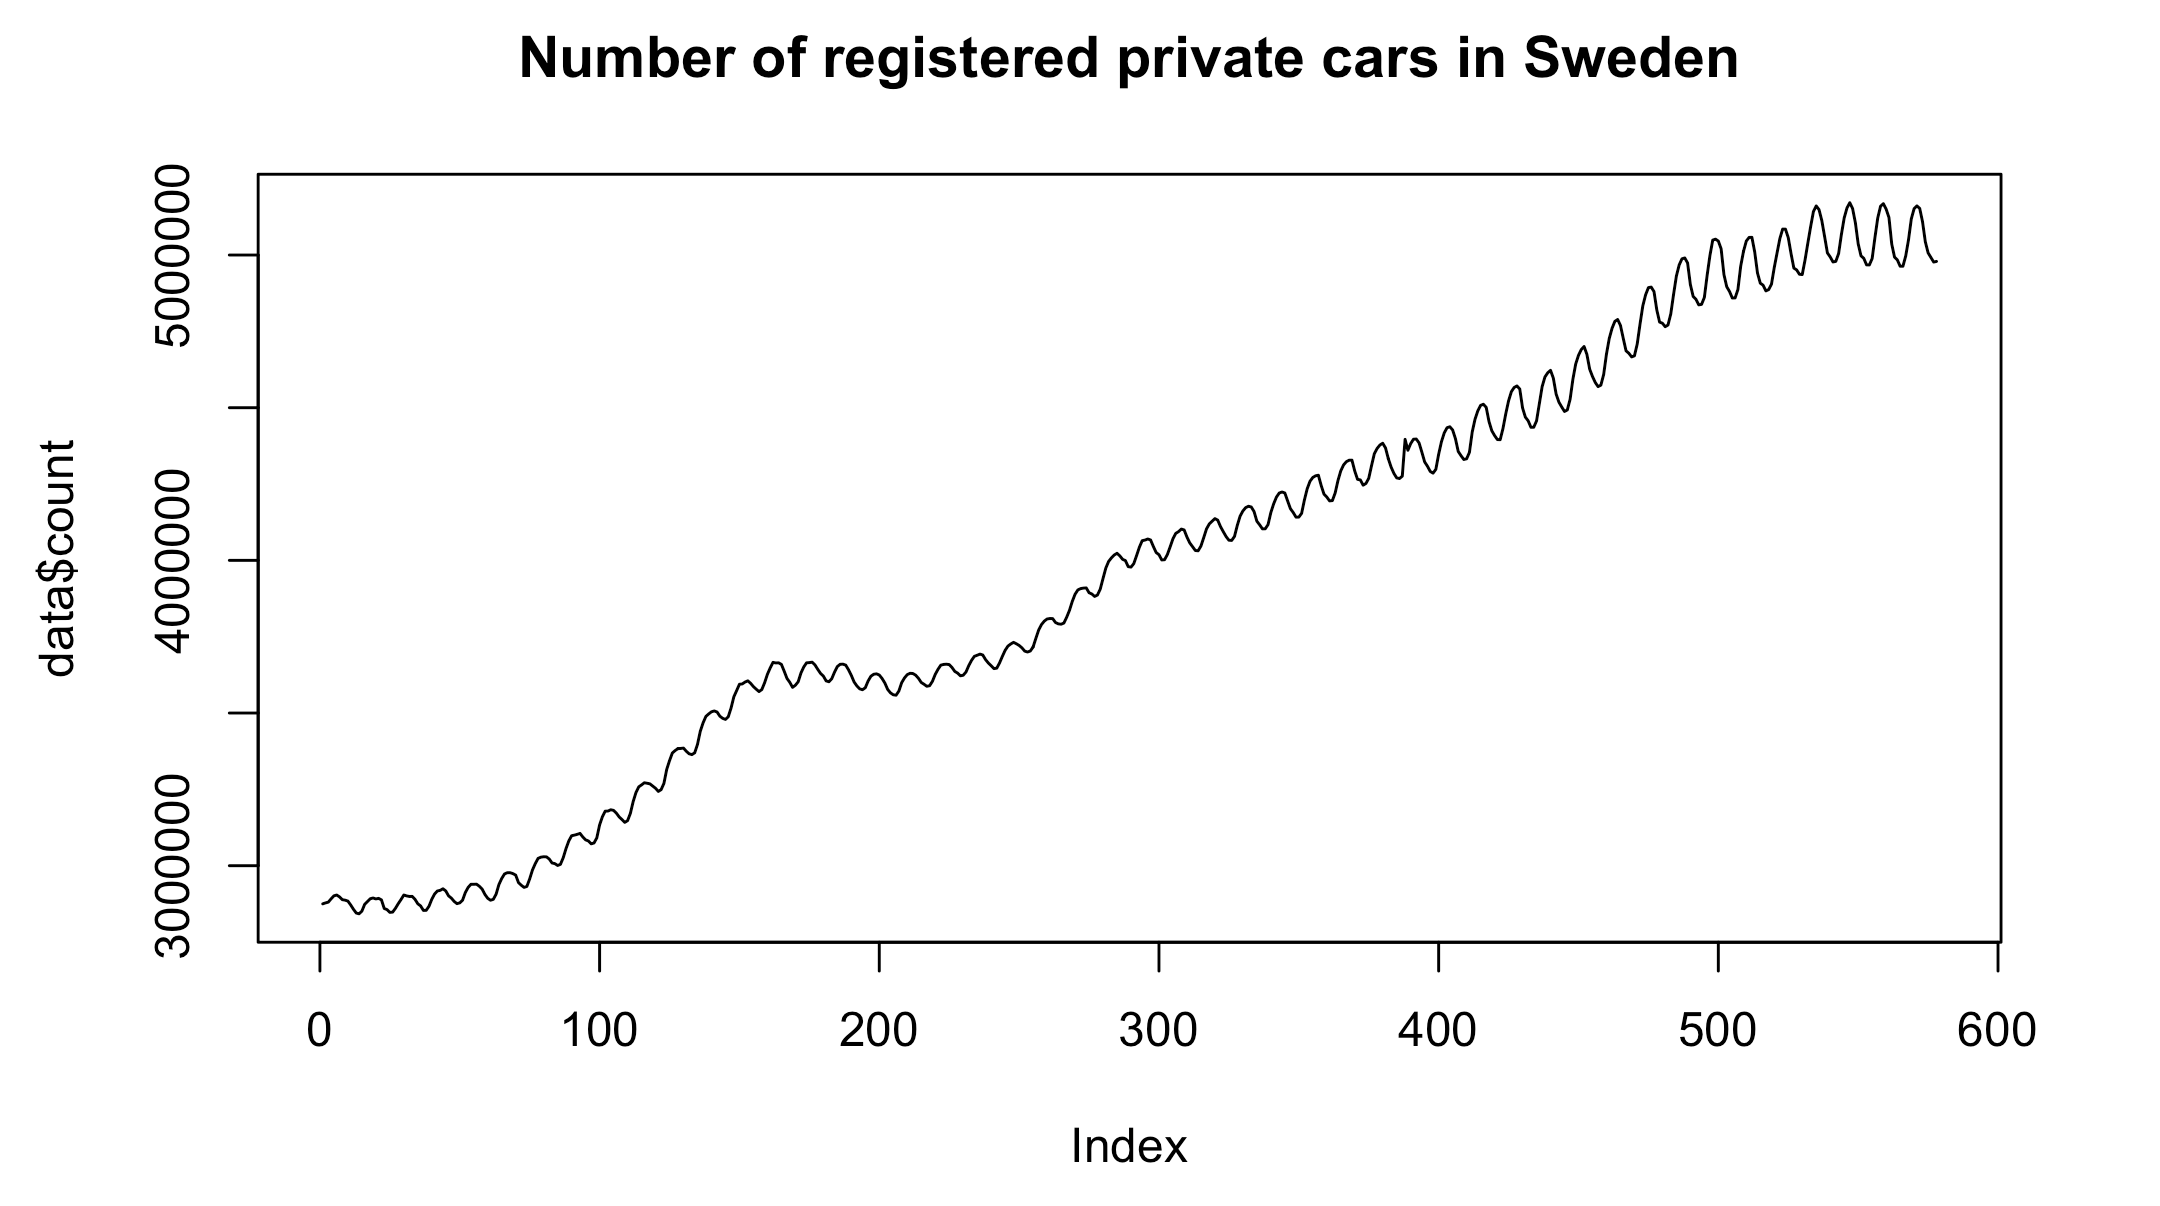
\includegraphics[width=1\textwidth]{carsmon-tsplot.png}
        \label{fig:f1}
    \end{figure}

    As the mean of the data with respect to time is changing, along with slight differences in the variance noticeable after around index 350, the data appears to be non-stationary initially. Upon applying a log transformation, to reduce the magnitude of the variance, and to scale down the data, the graph looks like the following:

    \begin{figure}[H]
        \centering
        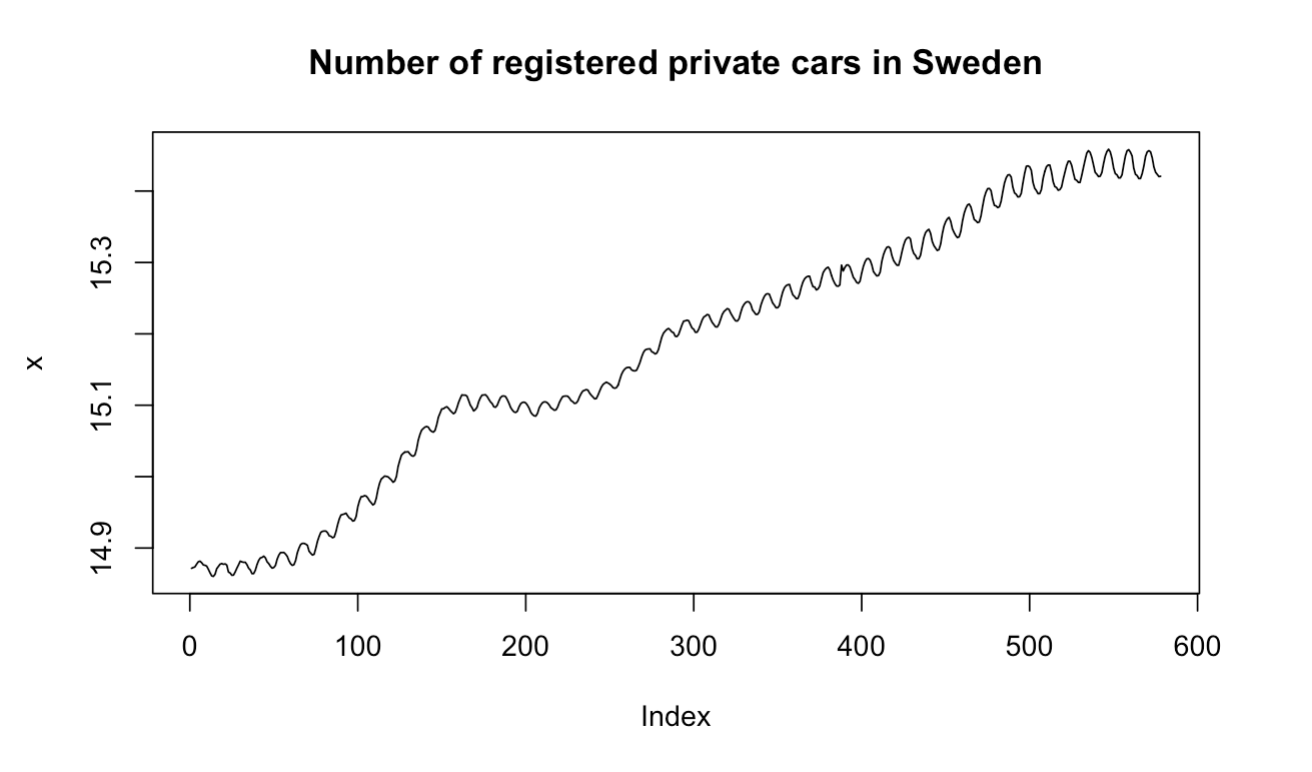
\includegraphics[width=1\textwidth]{log-transformed.png}
        \label{fig:f2}
    \end{figure}

    \bibliographystyle{unsrt}
    \bibliography{references}

    \newpage
    \appendix
    \section{Code}
    \lstinputlisting[language=R, caption=This is a code block.]{code.r}
\end{document}